%    File:    distance-measurements.tex
%    Author:  Marvin Smith
%    Date:    11/20/2015
%



%--------------------------------------------------%
%-       Start of Coordinate Conversions          -%
%--------------------------------------------------%
\addcontentsline{toc}{section}{Distance Measurements}
\section*{Distance Measurements}

Computing the distance between two points is yet another unique challenge in 
Geography.  To many, computing distance on a map seems like a simple problem. 
In Cartesian coordinates, the most often used metric is the \emph{Distance Formula}.

Given $P_1 (X,Y)$ and $P_2 (X,Y)$, the Cartesian distance is simply,
\begin{equation}
d = \sqrt{ \left(P_{2_x} - P_{1_x} \right)^2 + \left(P_{2_y} - P_{1_y} \right)^2}
\end{equation}

or more formally, given N-dimensional coordinates $P_1$ and $P_2$,

\begin{equation}
d = \sqrt{ \sum^{N}_{i=1} (P_{2_i} - P_{1_i} )^2}
\end{equation}


The issue with Cartesian coordinates is that they are only appropriate for certain
conditions.  Geographic (lat/lon) uses a spherical coordinate system which represents positions
in angles from the origin, not distance from the origin.  In figure \ref{fig:ortho_vs_merc}, 
the differences in routes between the two same points can be observed between
an orthographic and mercator projection.

\begin{figure}[!h]
\begin{subfigure}[b]{3in}
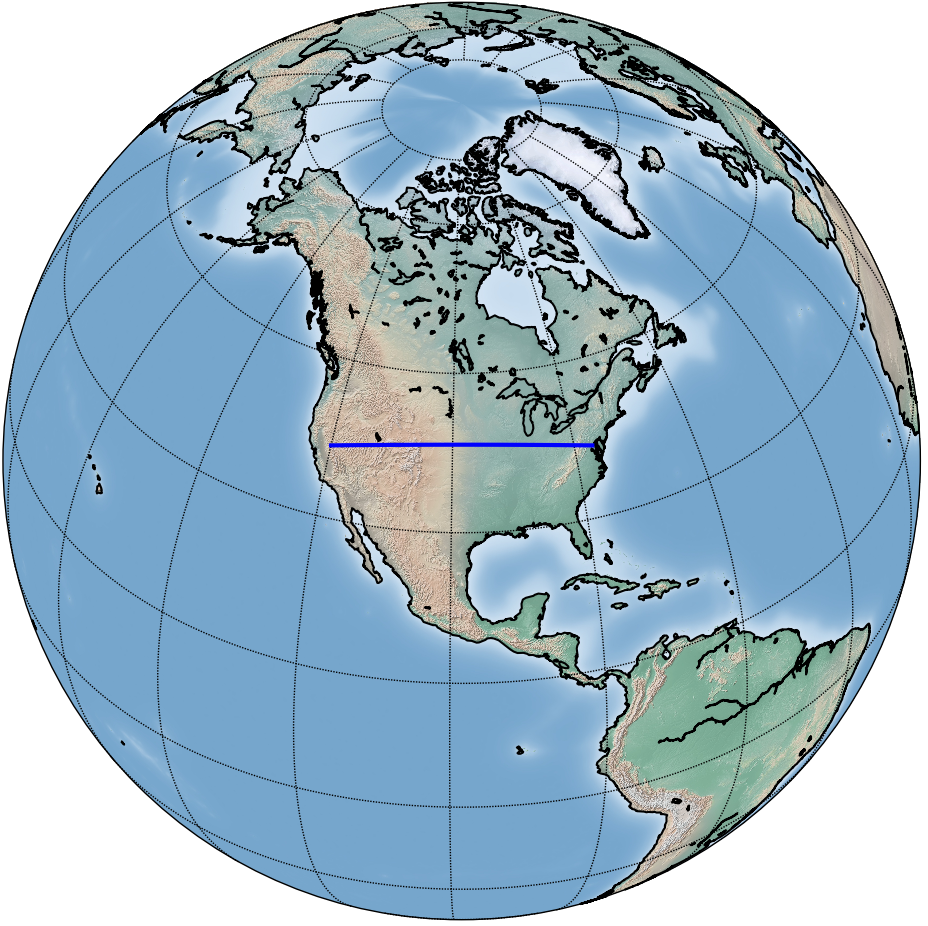
\includegraphics[width=3in]{chapter3/diagrams/figure_1.png}
\end{subfigure}
\begin{subfigure}[b]{3in}
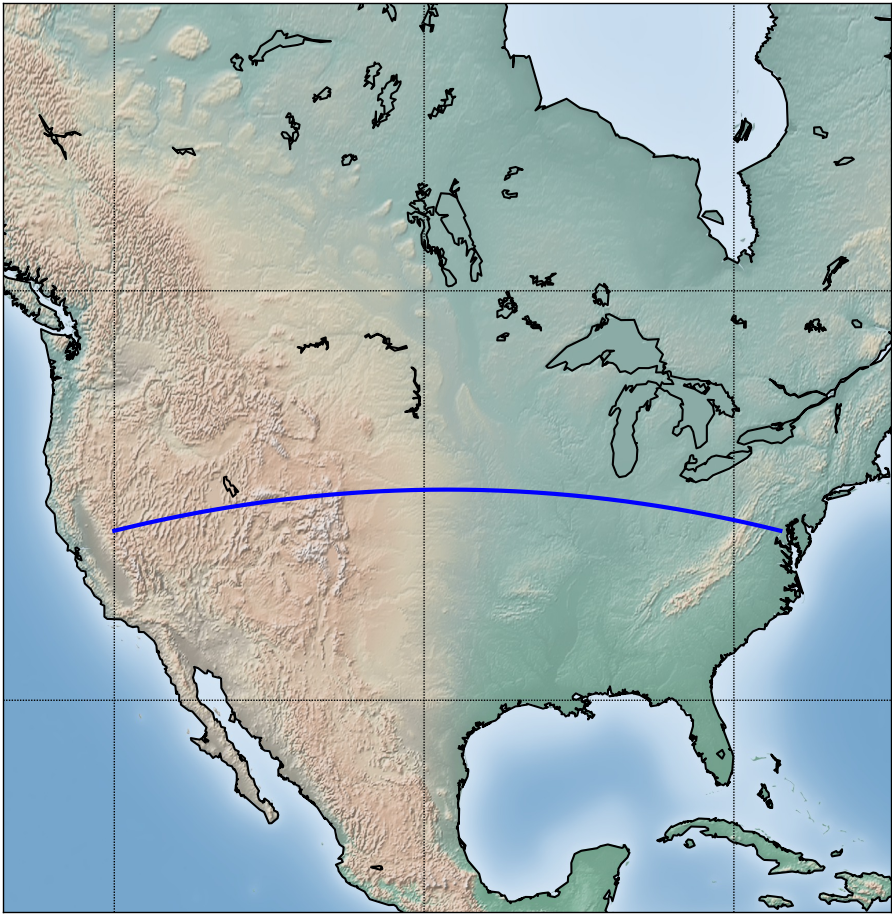
\includegraphics[width=3in]{chapter3/diagrams/figure_2.png}
\end{subfigure}
\caption{Orthographic vs. Mercator Projection for line between (39,-120) to (39,-77)}
\label{fig:ortho_vs_merc}
\end{figure}


\addcontentsline{toc}{subsection}{Coordinate Distances for Geographic Coordinates}
\subsection*{Coordinate Distances for Geographic Coordinates}


\addcontentsline{toc}{subsubsection}{Great Circle Distances}
\subsubsection*{Great Circle Distances}

The \emph{Great Circle} is the intersection of a plane with a sphere.  This intersection
results in a circle which represents the shortest distance between any two points on
a sphere\cite[p. 108]{Meyer_Book}.  This section is not meant to provide a useful navigational aid, but rather to 
provide the user with a simple computational example.  Great Circle distances are no longer popular in GIS
as Datums are now in Ellipsoids and computational performance now renders the usefulness less relevant. A 
popular equation for this is the \emph{Haversine} formula.  Avoid the technical great circle equation as
it does not perform well under small distances.

The equation is given where Latitude is $phi$, Longitude is $\lambda$, and the Earth's radius is $r$.

\begin{equation}
d_{gc} = 2r \arcsin \left( \sqrt{ \sin^2 \frac{\phi_2 - \phi_1}{2} + \cos{\phi_1} + \cos{\phi_2} \sin^2 \left( \frac{\lambda_2 - \lambda_1}{2} \right) }  \right)
\end{equation}

Here is a C++ example of the Haversine equation. This example was derived partially from \cite[p. 109]{Meyer_Book}.
\inputminted{C++}{../code/chapter3/great-circle-distance.cpp}

\addcontentsline{toc}{subsubsection}{Geodesic Ellipsoid Distances}
\subsubsection*{Geodesic Ellipsoid Distances}


GeographicLib once again is a useful utility for Geodesic distances.  

\inputminted{C++}{../code/chapter3/geographiclib-ellipsoid-distance.cpp}




\addcontentsline{toc}{subsubsection}{Projected Coordinate Distances}
\subsubsection*{Projected Coordinate Distances}


